\documentclass[a4paper,11pt]{book}
%\documentclass[a4paper,twoside,11pt,titlepage]{book}
\usepackage{listings}
\usepackage[utf8]{inputenc}
\usepackage[spanish]{babel}

% \usepackage[style=list, number=none]{glossary} %
%\usepackage{titlesec}
%\usepackage{pailatino}

\decimalpoint
\usepackage{dcolumn}
\newcolumntype{.}{D{.}{\esperiod}{-1}}
\makeatletter
\addto\shorthandsspanish{\let\esperiod\es@period@code}
\makeatother


%\usepackage[chapter]{algorithm}
\RequirePackage{verbatim}
%\RequirePackage[Glenn]{fncychap}
\usepackage{fancyhdr}
\usepackage{graphicx}
\usepackage{afterpage}
\usepackage{subfigure}
\usepackage{longtable}

\usepackage[pdfborder={000}]{hyperref} %referencia

% ********************************************************************
% Re-usable information
% ********************************************************************
\newcommand{\myTitle}{Título del proyecto\xspace}
\newcommand{\myDegree}{Grado en ...\xspace}
\newcommand{\myName}{Nombre Apllido1 Apellido2 (alumno)\xspace}
\newcommand{\myProf}{Nombre Apllido1 Apellido2 (tutor1)\xspace}
\newcommand{\myOtherProf}{Nombre Apllido1 Apellido2 (tutor2)\xspace}
%\newcommand{\mySupervisor}{Put name here\xspace}
\newcommand{\myFaculty}{Escuela Técnica Superior de Ingenierías Informática y de
Telecomunicación\xspace}
\newcommand{\myFacultyShort}{E.T.S. de Ingenierías Informática y de
Telecomunicación\xspace}
\newcommand{\myDepartment}{Departamento de ...\xspace}
\newcommand{\myUni}{\protect{Universidad de Granada}\xspace}
\newcommand{\myLocation}{Granada\xspace}
\newcommand{\myTime}{\today\xspace}
\newcommand{\myVersion}{Version 0.1\xspace}


\hypersetup{
pdfauthor = {\myName (email (en) ugr (punto) es)},
pdftitle = {\myTitle},
pdfsubject = {},
pdfkeywords = {palabra_clave1, palabra_clave2, palabra_clave3, ...},
pdfcreator = {LaTeX con el paquete ....},
pdfproducer = {pdflatex}
}

%\hyphenation{}


%\usepackage{doxygen/doxygen}
%\usepackage{pdfpages}
\usepackage{url}
\usepackage{colortbl,longtable}
\usepackage[stable]{footmisc}
%\usepackage{index}

%\makeindex
%\usepackage[style=long, cols=2,border=plain,toc=true,number=none]{glossary}
% \makeglossary

% Definición de comandos que me son tiles:
%\renewcommand{\indexname}{Índice alfabético}
%\renewcommand{\glossaryname}{Glosario}

\pagestyle{fancy}
\fancyhf{}
\fancyhead[LO]{\leftmark}
\fancyhead[RE]{\rightmark}
\fancyhead[RO,LE]{\textbf{\thepage}}
\renewcommand{\chaptermark}[1]{\markboth{\textbf{#1}}{}}
\renewcommand{\sectionmark}[1]{\markright{\textbf{\thesection. #1}}}
\renewcommand\lstlistingname{Listado}

\setlength{\headheight}{1.5\headheight}

\newcommand{\HRule}{\rule{\linewidth}{0.5mm}}


\definecolor{pblue}{rgb}{0.13,0.13,1}
\definecolor{pgreen}{rgb}{0,0.5,0}
\definecolor{pred}{rgb}{0.9,0,0}
\definecolor{pgrey}{rgb}{0.46,0.45,0.48}


\lstset{language=Java,
	showspaces=false,
	showtabs=false,
	breaklines=true,
	showstringspaces=false,
	breakatwhitespace=true,
	commentstyle=\color{pgreen},
	keywordstyle=\color{pblue},
	stringstyle=\color{pred},
	basicstyle=\scriptsize\ttfamily,
	moredelim=[il][\textcolor{pgrey}]{$ $},
	moredelim=[is][\textcolor{pgrey}]{\%\%}{\%\%}
}

\lstset{literate=%
	{á}{{\'a}}1
	{é}{{\'e}}1
	{è}{{\`e}}1
	{í}{{\'i}}1
	{ó}{{\'o}}1
	{ú}{{\'u}}1
	{ñ}{{\~n}}1
}


\newcommand{\bigrule}{\titlerule[0.5mm]}


%Para conseguir que en las páginas en blanco no ponga cabecerass
\makeatletter
\def\clearpage{%
  \ifvmode
    \ifnum \@dbltopnum =\m@ne
      \ifdim \pagetotal <\topskip
        \hbox{}
      \fi
    \fi
  \fi
  \newpage
  \thispagestyle{empty}
  \write\m@ne{}
  \vbox{}
  \penalty -\@Mi
}
\makeatother

\usepackage{pdfpages}
\usepackage{datetime}
\usepackage{geometry,calc}
\usepackage{caption}
\usepackage{csquotes}
\usepackage{algorithm}
\usepackage{algpseudocode}
\usepackage{amsmath}
%%%%%%%%%%%%%%%%%%%%%%%%%%%%%%%%%%%%%%%%%
% Short Sectioned Assignment LaTeX Template Version 1.0 (5/5/12)
% This template has been downloaded from: http://www.LaTeXTemplates.com
% Original author:  Frits Wenneker (http://www.howtotex.com)
% License: CC BY-NC-SA 3.0 (http://creativecommons.org/licenses/by-nc-sa/3.0/)
%%%%%%%%%%%%%%%%%%%%%%%%%%%%%%%%%%%%%%%%%

%----------------------------------------------------------------------------------------
%	PACKAGES AND OTHER DOCUMENT CONFIGURATIONS
%----------------------------------------------------------------------------------------

% ---- Entrada y salida de texto -----

\usepackage[T1]{fontenc} % Use 8-bit encoding that has 256 glyphs
\usepackage[utf8]{inputenc}
%\usepackage{fourier} % Use the Adobe Utopia font for the document - comment this line to return to the LaTeX default

% ---- Idioma --------

\usepackage[spanish, es-tabla]{babel} % Selecciona el español para palabras introducidas automáticamente, p.ej. "septiembre" en la fecha y especifica que se use la palabra Tabla en vez de Cuadro

% ---- Otros paquetes ----

%https://en.wikibooks.org/wiki/LaTeX/Hyperlinks#.5Curl
\usepackage[colorlinks=true,linkcolor=blue,citecolor=red, urlcolor=blue]{hyperref} % para poder poner referencias, url...

%https://en.wikibooks.org/wiki/LaTeX/Colors
\usepackage{color, colortbl}
\usepackage[first=0,last=9]{lcg} %Color tabla
\newcommand{\ra}{\rand0.\arabic{rand}} %Color tabla


\usepackage{eurosym} %Símbolo del euro

\usepackage{amsmath,amsfonts,amsthm} % Math packages
%\usepackage{graphics,graphicx, floatrow} %para incluir imágenes y notas en las imágenes
\usepackage{graphics,graphicx, float, url} %para incluir imágenes y colocarlas

% Para hacer tablas comlejas
%\usepackage{multirow}
%\usepackage{threeparttable}

%\usepackage{sectsty} % Allows customizing section commands
%\allsectionsfont{\centering \normalfont\scshape} % Make all sections centered, the default font and small caps

\usepackage{fancyhdr} % Custom headers and footers
\pagestyle{fancyplain} % Makes all pages in the document conform to the custom headers and footers
\fancyhead{} % No page header - if you want one, create it in the same way as the footers below
\fancyfoot[L]{} % Empty left footer
\fancyfoot[C]{} % Empty center footer
\fancyfoot[R]{\thepage} % Page numbering for right footer
\renewcommand{\headrulewidth}{0pt} % Remove header underlines
\renewcommand{\footrulewidth}{0pt} % Remove footer underlines
\setlength{\headheight}{13.6pt} % Customize the height of the header
\usepackage{pdfpages}
\numberwithin{equation}{section} % Number equations within sections (i.e. 1.1, 1.2, 2.1, 2.2 instead of 1, 2, 3, 4)
\numberwithin{figure}{section} % Number figures within sections (i.e. 1.1, 1.2, 2.1, 2.2 instead of 1, 2, 3, 4)
\numberwithin{table}{section} % Number tables within sections (i.e. 1.1, 1.2, 2.1, 2.2 instead of 1, 2, 3, 4)

\setlength\parindent{0pt} % Removes all indentation from paragraphs - comment this line for an assignment with lots of text

\newcommand{\horrule}[1]{\rule{\linewidth}{#1}} % Create horizontal rule command with 1 argument of height

\begin{document}
\begin{titlepage}
\newlength{\centeroffset}
\setlength{\centeroffset}{-0.5\oddsidemargin}
\addtolength{\centeroffset}{0.5\evensidemargin}
\thispagestyle{empty}

\noindent\hspace*{\centeroffset}\begin{minipage}{\textwidth}

\centering

\includegraphics[width=0.9\textwidth]{imagenes/logo_ugr.jpg}\\[1.4cm]

\textsc{ \Large PRÁCTICA PROCESOS GAUSSIANOS\\[0.2cm]}
\textsc{ Máster DATCOM }\\[1cm]
% Upper part of the page
% 
% Title
{\Huge\bfseries Extracción de Características en Imágenes\\
}
\noindent\rule[-1ex]{\textwidth}{3pt}\\[3.5ex]
{\large\bfseries }
\end{minipage}

\vspace{1cm}
\noindent\hspace*{\centeroffset}\begin{minipage}{\textwidth}
\centering

\textbf{Autor}\\ {Alberto Armijo Ruiz}\\[2.5ex]

\includegraphics[width=0.3\textwidth]{imagenes/etsiit_logo.png}\\[0.1cm]
\textsc{Escuela Técnica Superior de Ingenierías Informática y de Telecomunicación}\\
\textsc{---}\\
\today
\end{minipage}
%\addtolength{\textwidth}{\centeroffset}
%\vspace{\stretch{2}}
\end{titlepage}
\chapter*{}
\section{Resumen}
En esta práctica se realizará un estudio sobre diferentes tipos de descriptores de imágenes; en concreto HOG (Histogram of Gradients) y LBP (Local Binary Patterns). De este último se realizará una modificación, para cuál también se realizará un estudio con diferentes clasificadores. Por último, se describirá el proceso para crear un detector de personas en imágenes con uno de los clasificadores generados en los apartados anteriores y se analizarán los resultados que produce. \\

Esta práctica ha sido realizada en Python 3 junto con OpenCV. Dentro del fichero comprimido se encontrarán los diferentes archivos con la implementación de los descriptores, los archivos de pruebas, el archivo con los resultados, y el archivo que contiene la implementación del detector de personas. Adicionalmente se proporcionan archivos con los datos generados por los descriptores comprimidos ya que tardan bastante en cargarse de forma normal por si se desea ejecutar las pruebas con los diferentes descriptores.

%\frontmatter
\tableofcontents
\listoffigures
\listoftables
%
%\mainmatter
%\setlength{\parskip}{5pt}

\chapter{Evaluación del descriptor HOG}
Para esta primera parte de la práctica se realizará un análisis de los resultados obtenidos con el descriptor HOG (Histogram of Gradients), para ello, se definirán diferentes funciones, tanto para entrenar el modelo y obtener resultados como para hacer validación cruzada. El contenido que se va a explicar a continuación se encuentra dentro de los archivos \textbf{Extracción de rasgos.py} y \textbf{pruebas\_hog.py}.

\section{Lectura de imágenes,creación del modelo y predicción con nuevas imágenes}
Lo primero que se debe hacer es leer los datos, para ello se ha creado la función \textit{loadTrainingData()}, esta función se encarga de abrir cada una de las imágenes contenidas en la carpeta de train que se proporciona con la práctica de ejemplo \textit{ECI.Practica}; por cada una de la imágenes se computa se descriptor HOG; para ello se hace uso de la función \textit{cv2.HOGDescriptor().compute()}. \\

Para esta práctica se está utilizando un descriptor HOG con parámetros por defecto; este descriptor por defecto utiliza un tamaño de ventana de 128x64, bloques de 16x16, desplazamientos de 8x8, ... Con estos parámetros obtenemos por cada ventana 3780 características. Las imágenes que se utilizan en esta práctica son de 128x64, por lo que al utilizar el descriptor sobre estas cada una producirá un vector con 3780 características. Además de computar el descriptor por cada una de las imágenes, se añaden también a un vector la clase a la que pertenece cada imagen; dicho vector contiene unos (imágenes con personas en las fotos) y ceros (imágenes con fondo, sin personas). Una vez se han generado todas las imágenes se devuelve una matriz que contiene todos los descriptores calculados y un vector con la clase de cada imagen. \\

Tras esto, se debe entrenar un modelo para después poder predecir clases de una imagen dada; para ello, se utilizará como clasificador un \textit{SVM} contenido en la librería de \textit{OpenCV}. Este clasificador permite utilizar diferentes tipos de ``kernels`` que se utilizan después para realizar transformaciones a los datos y conseguir una mejor separación de estos; por el momento se va a utilizar un kernel lineal, más tarde se realizarán pruebas con diferentes kernels y se analizarán los resultados obtenidos.\\

Para utilizar este clasificador es necesario utilizar la función \textit{cv.ml.SVM\_create()}, esta función nos genera un \textit{SVM} vacío al que le podemos aplicar los parámetros que queramos, por defecto se definirá el tipo de kernel (lineal) y el tipo de SVM (en este caso de clasificación); también se le pueden (o deben) añadir más parámetros dependiendo del tipo de kernel que se utilice. Una vez definidos dichos parámetros del \textit{SVM} se utiliza la función \textit{train()} a la que se le pasa la matriz de descriptores, el vector de clases de las imágenes y además se le añade un parámetro indicando si las filas son los ejemplos o son las columnas (en el caso de esta práctica son las filas las que contienen cada uno de los ejemplos). Todo esto está contenido dentro de la función \textit{train()}, definida dentro de la práctica, a la cual se le pasa la matriz de descriptores, el vector de clases, el tipo de kernel que utilizará el clasificador, y un parámetro llamado ``degree`` utilizado por algunos kernels. \\

Una vez se ha entrenado el modelo, podemos utilizarlo para predecir la clase de una imagen. Para ello se ha creado la función \textit{test()}, a la cual se le pasa una imagen y el clasificador que queremos utilizar. Para la imagen dada se computa su descriptor HOG; tras esto, se utiliza la función \textit{clasficador.predict()} para obtener la predicción; este método nos devuelve una tupla, de la cual nos interesa el segundo valor de esta, en la cual se encuentra un vector con la clase predicha para la imagen; si se utilizara la función \textit{clasificador.predict()} sobre varios descriptores, este vector contendría la clase predicha para cada uno de los descriptores. \\

El proceso de crear leer las imágenes, crear un modelo y realizar una prueba con una imagen esta contenido dentro de la función \textit{ejemploClasificadorImagenes()} dentro de este ejemplo se utiliza como test una imagen de una persona, por lo que el resultado de la predicción debe de ser uno. A continuación se mostrará la imagen utilizada y una foto con la salida de la función. \\

\newpage

\begin{figure}[H]
	\centering
	\subfigure{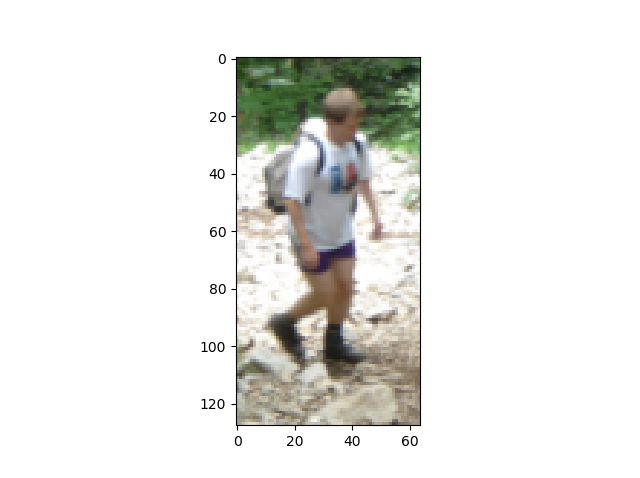
\includegraphics[width=80mm]{imagenes/prueba_img}}
	\subfigure{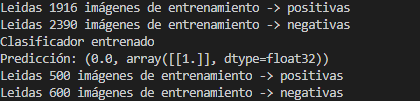
\includegraphics[width=80mm]{imagenes/resultado_ini}}
	\caption{Ejemplo clasificación con SVM lineal}
	\label{fig:salida_1}
\end{figure}

\section{Cálculo de medidas de interés para HOG}
En este apartado, se describirá el proceso realizado para obtener medidas de interés sobre el clasificador, para ello se cargará un conjunto de imágenes de test y se creará una función para calcular diferentes medidas de interés. \\

Para cargar el conjunto de imágenes de test se realiza el mismo proceso que en el apartado anterior, pero en vez de computar el descriptor para estas imágenes se guardan las imágenes; esto se realiza en la función \textit{loadTestData()}. Tras esto se utiliza la función \textit{test()} sobre cada una de las imágenes y se obtienen las predicciones del clasificador. Una vez se han obtenido las predicciones estás se guardan en un vector y se utiliza la función \textit{calculateMetrics()} para obtener las diferentes medidas. \\

La función \textit{calculateMetrics()} se encarga de obtener medidas de interés para los datos que se predicen, dichas medidas son \textit{F1-score}, \textit{Accuracy}, \textit{Precision}, \textit{True Negative Rate}, \textit{True Positive Rate}.A esta función se le debe pasar la predicción hecha por el clasificador y la clase real de los datos. Dichas medidas miden lo siguiente:
\begin{itemize}
	\item \textbf{Accuracy:} mide el porcentaje de predicciones correctas sobre el total de predicciones realizadas.
	\item \textbf{Precision:} mide el porcentaje de predicciones positivas reales sobre el total de predicciones positivas realizadas, es decir, el porcentaje de imágenes que se han clasificado como positivas que realmente son positivas.
	\item \textbf{True Positive Rate:} mide el porcentaje de predicciones positivas hechas sobre el total de datos positivos que hay, es decir, el porcentaje de imágenes positivas que se han clasificado como positivas.
	\item \textbf{True Negative Rate:} mide el porcentaje de predicciones negativas hechas sobre el total de datos negativos que hay, es decir, el porcentaje de imágenes negativas que se han clasificado como negativas.
	\item \textbf{F1-score:} está medida calcula una proporción entre \textit{Precision} y \textit{True Positive Rate}, indica la calidad de la predicción de la clase positiva, en nuestro caso sería detectar a una persona en la imagen. Esta medida decrece sin cualquiera de las dos medidas anteriores decrece.
\end{itemize}

Estas medidas nos serán útiles para conocer mejor como se está ajustando el clasificador entrenado con los datos. Los resultados obtenidos para nuestro conjunto de test son los siguientes.
\begin{figure}[H]
	\centering
	
\includegraphics[width=140mm]{imagenes/resultados_test}
	\caption{Resultados de test para HOG}
	\label{fig:salida_2}
\end{figure}

Como se puede ver, los resultados son bastante buenos, obteniendo un 96\% aproximado de acierto, como se puede ver en el resto de medidas, el clasificador ha obtenido mejores resultados clasificando imágenes como fondo que como persona, aunque realmente no hay mucha diferencia.

\section{Pruebas con HOG}
En este apartado se compararán diferentes clasificadores a través de las medidas de interés descritas en el apartado anterior. Para este apartado se han utilizado todas las imágenes, en total 5406, y se ha utilizado validación cruzada para crear diferentes conjuntos de validación, de esta forma se pueden ver resultados más generales que no dependan solamente de los resultados de un único conjunto de validación y estar más seguros de la calidad del clasificador.\\

Para realizar validación cruzada se ha creado la función \textit{crossValidation()} esta función tiene como parámetros la matriz de datos con los descriptores, el vector de clases de dichos casos y el número de validaciones a realizar, por defecto este último parámetro es 5, el cual es el número de validaciones que se han utilizado para realizar el estudio de los diferentes clasificadores. También tiene parámetros adicionales para poder definir las características del clasificador. Dentro de esta función se realiza el siguiente proceso por cada validación.
\begin{enumerate}
	\item Se crea un conjunto de datos de validación. Para ello se utiliza la función de la librería \textit{sklearn.train\_test\_split()}; dicha función nos divide el conjunto de datos en un conjunto de datos de train y otro de test; para ello elige de forma aleatoria cada vez un conjunto de datos para test y forma el conjunto de train sin incluir dichos datos. Para el estudio se ha utilizado un tamaño de train del 80\% de los datos y un 20\% para test.
	\item Se crea un modelo y se entrena con el conjunto de datos de test.
	\item Se obtienen las predicciones de este modelo para los datos de test, se calculan la medidas anteriormente descritas y se guardan.
	\item Se actualiza el mejor modelo obtenido hasta el modelo, para ello se utiliza la medida \textit{Accuracy}; esto nos será útil para guardar el mejor modelo encontrado para la validación y utilizarlo más tarde si es necesario.
\end{enumerate}


Ahora, pasaremos a comentar los resultados obtenidos por el descriptor HOG con diferentes kernels de SVM y variando algunos parámetros. Los clasificadores que se han entrenado son los siguientes: SVM con kernel lineal, SVM con kernel radial (RBF), SVM con kernel polinómico con grados 2, 3, 4 y 5, SVM con kernel sigmoidal, SVM con kernel Chi Cuadrado y SVM con kernel Inter. Para cada uno de los modelo se han realizado 5 validaciones. Los parámetros a excepción de los diferentes clasificadores son los que hay por defecto; esto se ha hecho así para evitar ajustar los parámetros a un tipo de descriptor, ya que con otros descriptores; como los que se verán más adelante, los resultados pueden no ser justos por dichos parámetros .Los resultados son los siguientes:

\vspace{0.09in}

\begin{table}[H]
	\begin{tabular}{llllll}
		\textbf{Validation} & \textbf{F1} & \textbf{accuracy} & \textbf{precision} & \textbf{truenegativerate} & \textbf{truepositiverate} \\
		0                   & 0.955533    & 0.960259          & 0.966527           & 0.973019                  & 0.944785                  \\
		1                   & 0.960566    & 0.963956          & 0.979381           & 0.982699                  & 0.942460                  \\
		2                   & 0.959474    & 0.965804          & 0.962637           & 0.972756                  & 0.956332                  \\
		3                   & 0.953751    & 0.958410          & 0.960663           & 0.967905                  & 0.946939                  \\
		4                   & 0.970854    & 0.973198          & 0.979716           & 0.982759                  & 0.962151                 
	\end{tabular}
	\caption{Validación con SVM kernel lineal}
	\label{table_1}
\end{table}

\begin{table}[H]
	\begin{tabular}{llllll}
		\textbf{Validation} & \textbf{F1} & \textbf{accuracy} & \textbf{precision} & \textbf{truenegativerate} & \textbf{truepositiverate} \\
		0                   & 0.853179    & 0.882625          & 0.960938           & 0.975042                  & 0.767152                  \\
		1                   & 0.834146    & 0.874307          & 0.957983           & 0.975767                  & 0.738661                  \\
		2                   & 0.850123    & 0.887246          & 0.971910           & 0.983974                  & 0.755459                  \\
		3                   & 0.854237    & 0.880776          & 0.952141           & 0.968013                  & 0.774590                  \\
		4                   & 0.865106    & 0.888170          & 0.948655           & 0.964646                  & 0.795082                 
	\end{tabular}
	\caption{Validación con SVM kernel RBF}
	\label{table_2}
\end{table}

\begin{table}[H]
	\begin{tabular}{llllll}
		\textbf{Validation} & \textbf{F1} & \textbf{accuracy} & \textbf{precision} & \textbf{truenegativerate} & \textbf{truepositiverate} \\
		0                   & 0.963441    & 0.968577          & 0.976035           & 0.981997                  & 0.951168                  \\
		1                   & 0.969008    & 0.972274          & 0.985294           & 0.988136                  & 0.953252                  \\
		2                   & 0.973601    & 0.976895          & 0.976695           & 0.981878                  & 0.970526                  \\
		3                   & 0.974039    & 0.976895          & 0.979123           & 0.983278                  & 0.969008                  \\
		4                   & 0.968442    & 0.970425          & 0.983968           & 0.985891                  & 0.953398                 
	\end{tabular}
\caption{Validación con SVM kernel polinómico grado 2}
\label{table_3}
\end{table}

\begin{table}[H]
	\begin{tabular}{llllll}
		\textbf{Validation} & \textbf{F1} & \textbf{accuracy} & \textbf{precision} & \textbf{truenegativerate} & \textbf{truepositiverate} \\
		0                   & 0.978238    & 0.980591          & 0.989518           & 0.991582                  & 0.967213                  \\
		1                   & 0.979955    & 0.983364          & 0.988764           & 0.992051                  & 0.971302                  \\
		2                   & 0.968153    & 0.972274          & 0.976445           & 0.981878                  & 0.960000                  \\
		3                   & 0.973577    & 0.975970          & 0.979550           & 0.982964                  & 0.967677                  \\
		4                   & 0.974722    & 0.976895          & 0.993814           & 0.994810                  & 0.956349                 
	\end{tabular}
\caption{Validación con SVM kernel polinómico grado 3}
\label{table_4}
\end{table}

\begin{table}[H]
	\begin{tabular}{llllll}
		\textbf{Validation} & \textbf{F1} & \textbf{accuracy} & \textbf{precision} & \textbf{truenegativerate} & \textbf{truepositiverate} \\
		0                   & 0.970684    & 0.975046          & 0.984581           & 0.988618                  & 0.957173                  \\
		1                   & 0.969325    & 0.972274          & 0.983402           & 0.986348                  & 0.955645                  \\
		2                   & 0.981289    & 0.983364          & 0.995781           & 0.996633                  & 0.967213                  \\
		3                   & 0.973188    & 0.975046          & 1.000000           & 1.000000                  & 0.947776                  \\
		4                   & 0.972860    & 0.975970          & 0.991489           & 0.993266                  & 0.954918                 
	\end{tabular}
\caption{Validación con SVM kernel polinómico grado 4}
\label{table_5}
\end{table}

\begin{table}[H]
	\begin{tabular}{llllll}
		\textbf{Validation} & \textbf{F1} & \textbf{accuracy} & \textbf{precision} & \textbf{truenegativerate} & \textbf{truepositiverate} \\
		0                   & 0.970982    & 0.975970          & 0.981941           & 0.987281                  & 0.960265                  \\
		1                   & 0.973568    & 0.977819          & 0.988814           & 0.991948                  & 0.958785                  \\
		2                   & 0.971904    & 0.975046          & 0.991507           & 0.993243                  & 0.953061                  \\
		3                   & 0.972399    & 0.975970          & 0.982833           & 0.986799                  & 0.962185                  \\
		4                   & 0.966135    & 0.968577          & 0.981781           & 0.984266                  & 0.950980                 
	\end{tabular}
\caption{Validación con SVM kernel polinómico grado 5}
\label{table_6}
\end{table}

\begin{table}[H]
	\begin{tabular}{llllll}
		\textbf{Validation} & \textbf{F1} & \textbf{accuracy} & \textbf{precision} & \textbf{truenegativerate} & \textbf{truepositiverate} \\
		0                   & 0.530194    & 0.575786          & 0.531828           & 0.614865                  & 0.528571                  \\
		1                   & 0.531154    & 0.575786          & 0.521042           & 0.602990                  & 0.541667                  \\
		2                   & 0.617252    & 0.446396          & 0.446396           & 0.000000                  & 1.000000                  \\
		3                   & 0.535865    & 0.593346          & 0.541578           & 0.643449                  & 0.530271                  \\
		4                   & 0.520686    & 0.560998          & 0.503906           & 0.578773                  & 0.538622                 
	\end{tabular}
\caption{Validación con SVM kernel sigmoidal}
\label{table_7}
\end{table}

\begin{table}[H]
	\begin{tabular}{llllll}
		\textbf{Validation} & \textbf{F1} & \textbf{accuracy} & \textbf{precision} & \textbf{truenegativerate} & \textbf{truepositiverate} \\
		0                   & 0.698479    & 0.597043          & 0.539530           & 0.246503                  & 0.990196                  \\
		1                   & 0.651129    & 0.557301          & 0.489059           & 0.250401                  & 0.973856                  \\
		2                   & 0.661839    & 0.568392          & 0.500000           & 0.256911                  & 0.978587                  \\
		3                   & 0.670968    & 0.575786          & 0.506494           & 0.253682                  & 0.993631                  \\
		4                   & 0.684507    & 0.585952          & 0.524838           & 0.251701                  & 0.983806                 
	\end{tabular}
\caption{Validación con SVM kernel Chi Cuadrado}
\label{table_8}
\end{table}

\begin{table}[H]
	\begin{tabular}{llllll}
		\textbf{Validation} & \textbf{F1} & \textbf{accuracy} & \textbf{precision} & \textbf{truenegativerate} & \textbf{truepositiverate} \\
		0                   & 0.970854    & 0.973198          & 0.977733           & 0.981067                  & 0.964072                  \\
		1                   & 0.975242    & 0.978743          & 0.997797           & 0.998353                  & 0.953684                  \\
		2                   & 0.976999    & 0.980591          & 0.986726           & 0.990338                  & 0.967462                  \\
		3                   & 0.977459    & 0.979667          & 0.987578           & 0.989813                  & 0.967546                  \\
		4                   & 0.988004    & 0.989834          & 0.993421           & 0.995169                  & 0.982646                 
	\end{tabular}
\caption{Validación con SVM kernel Inter}
\label{table_9}
\end{table}

Como se puede ver, el clasificador con kernel lineal obtiene buenos resultados de forma general, mejorando en una de sus validaciones a los resultados que se habían obtenido para test. Otros clasificadores como por el ejemplo el SVM con kernel RBF obtiene unos resultados algo peores, equivocándose bastante más que el clasificador con kernel lineal al clasificar personas. Otros clasificadores, como por ejemplo los que utilizan kernel polinómico o Inter obtienen resultados bastante parecidos a los obtenidos por el clasificador lineal. Por último, los clasificadores con kernel sigmoidal y Chi Cuadrado obtienen unos resultados bastante pobres, en el caso del primero no consigue diferenciar entre las clases y por ello obtiene resultados parecidos al de un clasificador aleatorio; en el caso del segundo clasificador se sobreajusta a los datos y elige en su mayoría de los datos como clase 1 (persona) por lo que se puede ver en la tabla (el \textit{True Positive Rate} es bastante alto mientras que \textit{Precision} no lo es).
\chapter{Clasificación con descriptor LBP}
En este apartado se describirá la clase \textit{LBP}, dicha clase implementa el funcionamiento del descriptor LBP. También se describirá el proceso necesario para obtener la matriz de descriptores generados con LBP. Por último se mostrarán los resultados obtenidos por diferentes modelos y se comentarán y compararán con los obtenidos con el descriptor HOG. La implementación del descriptor, el archivo pruebas se pueden encontrar en los ficheros \textbf{lbp.py} y \textbf{prueba\_lbp.py}; la función utilizada para cargar los datos en el fichero de pruebas y la función utilizada para computar el descriptor para cada una de las imágenes se pueden encontrar en el fichero \textbf{functions.py}

Si se desea ejecutar los ficheros de prueba para este descriptor o para los siguientes, se puede descargar un \textit{.zip} con los ficheros de clases y datos que los ficheros de pruebas cargan para hacer después las pruebas. El enlace es el siguiente: \url{https://drive.google.com/file/d/1fm0rdfdmWWLU8sjTXU59laeOh27URCDa/view?usp=sharing}

\section{Implementación del descriptor LBP}
Para la implementar el descriptor LBP se ha creado una clase, llamada \textit{LBP}. Dicha clase contiene el tamaño de la ventana, el número de vecinos a comparar y el tamaño de bloque. Dentro de esta clase se encuentra la función \textit{computeLBPpixel()} dicha función se encarga de comparar el valor de cada píxel con sus vecinos y de computar el valor LBP con los resultados obtenidos de la comparación. También se encuentra la función \textit{computeLBPblock()}, dicha función toma como argumentos la posición inicial del bloque y la imagen y computa el valor de cada pixel dentro de los límites del bloque. Por último tenemos la función \textit{computeLBPWindows()}, que toma como argumento la posición del primer píxel de la ventana y la imagen, con estos datos va llamando a la función descrita anteriormente hasta computar la ventana entera. También está la función \textit{compute()} a la cual se le pasa la imagen y esta llama \textit{computeLBPWindow()}. \\

\begin{figure}[H]
	\centering
	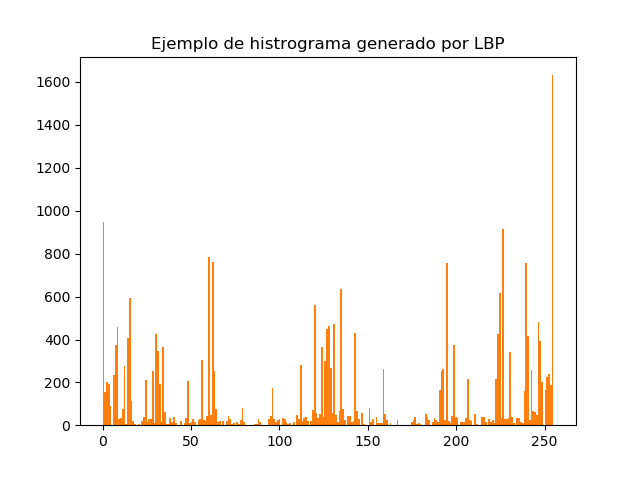
\includegraphics[width=140mm]{imagenes/lbp_histogram}
	\caption{Ejemplo Histograma de un descriptor LBP}
	\label{fig:salida_3}
\end{figure}

Una vez creada esta clase ya se pueden calcular los descriptores LBP para las imágenes. Para realizar la tarea de leer y computar los descriptores de la imágenes de forma general se ha implementado la función \textit{loadImages()} la cual toma de argumento un objeto de la clase del descriptor que se quiera utilizar siempre que su funcionamiento sea de la siguiente forma : descriptor.compute(imagen). Esta función se ha probado con HOG, la clase LBP implementada y la clase LBP-Uniforme, cuya descripción se encuentra en el siguiente apartado.

\section{Pruebas con LBP}
Para generar las validaciones con los diferentes modelos, se ha utilizado la función \textit{crossValidation()} (es la misma que se utiliza para el primer apartado) contenida en el archivo \textbf{functions.py}. Los resultados obtenidos son los siguientes:

\begin{table}[H]
	\begin{tabular}{llllll}
		\textbf{Validation} & \textbf{F1} & \textbf{accuracy} & \textbf{precision} & \textbf{truenegativerate} & \textbf{truepositiverate} \\
		0                   & 0.722057    & 0.740296          & 0.717092           & 0.751724                  & 0.727092                  \\
		1                   & 0.724521    & 0.747689          & 0.699805           & 0.745033                  & 0.751046                  \\
		2                   & 0.750000    & 0.767098          & 0.720000           & 0.754591                  & 0.782609                  \\
		3                   & 0.752753    & 0.771719          & 0.743083           & 0.779287                  & 0.762677                  \\
		4                   & 0.705385    & 0.742144          & 0.685832           & 0.754019                  & 0.726087                 
	\end{tabular}
	\caption{Validación con SVM kernel lineal}
	\label{table_10}
\end{table}

\begin{table}[H]
	\begin{tabular}{llllll}
		\textbf{Validation} & \textbf{F1} & \textbf{accuracy} & \textbf{precision} & \textbf{truenegativerate} & \textbf{truepositiverate} \\
		0                   & 0.609646    & 0.439002          & 0.438483           & 0.001645                  & 1.0                       \\
		1                   & 0.620778    & 0.450092          & 0.450092           & 0.000000                  & 1.0                       \\
		2                   & 0.612821    & 0.441774          & 0.441774           & 0.000000                  & 1.0                       \\
		3                   & 0.637681    & 0.468577          & 0.468085           & 0.001736                  & 1.0                       \\
		4                   & 0.611432    & 0.440850          & 0.440333           & 0.001650                  & 1.0                      
	\end{tabular}
	\caption{Validación con SVM kernel RBF}
	\label{table_11}
\end{table}

\begin{table}[H]
	\begin{tabular}{llllll}
		\textbf{Validation} & \textbf{F1} & \textbf{accuracy} & \textbf{precision} & \textbf{truenegativerate} & \textbf{truepositiverate} \\
		0                   & 0.757515    & 0.776340          & 0.744094           & 0.780405                  & 0.771429                  \\
		1                   & 0.742911    & 0.748614          & 0.711957           & 0.723958                  & 0.776680                  \\
		2                   & 0.752437    & 0.765250          & 0.735238           & 0.760757                  & 0.770459                  \\
		3                   & 0.738144    & 0.765250          & 0.720322           & 0.771757                  & 0.756871                  \\
		4                   & 0.754297    & 0.775416          & 0.732809           & 0.774086                  & 0.777083                 
	\end{tabular}
	\caption{Validación con SVM kernel polinómico grado 2}
	\label{table_12}
\end{table}

\begin{table}[H]
	\begin{tabular}{llllll}
		\textbf{Validation} & \textbf{F1} & \textbf{accuracy} & \textbf{precision} & \textbf{truenegativerate} & \textbf{truepositiverate} \\
		0                   & 0.762548    & 0.772643          & 0.745283           & 0.765625                  & 0.780632                  \\
		1                   & 0.769691    & 0.786506          & 0.745174           & 0.778894                  & 0.795876                  \\
		2                   & 0.753651    & 0.766174          & 0.706204           & 0.733002                  & 0.807933                  \\
		3                   & 0.763674    & 0.788355          & 0.728346           & 0.777778                  & 0.802603                  \\
		4                   & 0.768145    & 0.787431          & 0.750000           & 0.787625                  & 0.787190                 
	\end{tabular}
	\caption{Validación con SVM kernel polinómico grado 3}
	\label{table_13}
\end{table}

\begin{table}[H]
	\begin{tabular}{llllll}
		\textbf{Validation} & \textbf{F1} & \textbf{accuracy} & \textbf{precision} & \textbf{truenegativerate} & \textbf{truepositiverate} \\
		0                   & 0.347555    & 0.420518          & 0.352321           & 0.484034                  & 0.342916                  \\
		1                   & 0.359743    & 0.447320          & 0.365217           & 0.519737                  & 0.354430                  \\
		2                   & 0.288248    & 0.406654          & 0.311005           & 0.518395                  & 0.268595                  \\
		3                   & 0.727823    & 0.750462          & 0.691571           & 0.736928                  & 0.768085                  \\
		4                   & 0.373253    & 0.419593          & 0.349533           & 0.434146                  & 0.400428                 
	\end{tabular}
	\caption{Validación con SVM kernel polinómico grado 4}
	\label{table_14}
\end{table}

\begin{table}[H]
	\begin{tabular}{llllll}
		\textbf{Validation} & \textbf{F1} & \textbf{accuracy} & \textbf{precision} & \textbf{truenegativerate} & \textbf{truepositiverate} \\
		0                   & 0.613709    & 0.442699          & 0.442699           & 0.0                       & 1.0                       \\
		1                   & 0.612821    & 0.441774          & 0.441774           & 0.0                       & 1.0                       \\
		2                   & 0.624285    & 0.453789          & 0.453789           & 0.0                       & 1.0                       \\
		3                   & 0.623410    & 0.452865          & 0.452865           & 0.0                       & 1.0                       \\
		4                   & 0.624285    & 0.453789          & 0.453789           & 0.0                       & 1.0                      
	\end{tabular}
	\caption{Validación con SVM kernel polinómico grado 5}
	\label{table_15}
\end{table}

\begin{table}[H]
	\begin{tabular}{llllll}
		\textbf{Validation} & \textbf{F1} & \textbf{accuracy} & \textbf{precision} & \textbf{truenegativerate} & \textbf{truepositiverate} \\
		0                   & 0.619898    & 0.449168          & 0.449168           & 0.0                       & 1.0                       \\
		1                   & 0.626032    & 0.455638          & 0.455638           & 0.0                       & 1.0                       \\
		2                   & 0.609254    & 0.438078          & 0.438078           & 0.0                       & 1.0                       \\
		3                   & 0.607465    & 0.436229          & 0.436229           & 0.0                       & 1.0                       \\
		4                   & 0.629512    & 0.459335          & 0.459335           & 0.0                       & 1.0                      
	\end{tabular}
	\caption{Validación con SVM kernel sigmoidal}
	\label{table_16}
\end{table}

\begin{table}[H]
	\begin{tabular}{llllll}
		\textbf{Validation} & \textbf{F1} & \textbf{accuracy} & \textbf{precision} & \textbf{truenegativerate} & \textbf{truepositiverate} \\
		0                   & 0.619017    & 0.448244          & 0.448244           & 0.000000                  & 1.0                       \\
		1                   & 0.626429    & 0.456562          & 0.456059           & 0.001698                  & 1.0                       \\
		2                   & 0.625478    & 0.456562          & 0.455051           & 0.005076                  & 1.0                       \\
		3                   & 0.612323    & 0.441774          & 0.441258           & 0.001653                  & 1.0                       \\
		4                   & 0.609646    & 0.439002          & 0.438483           & 0.001645                  & 1.0                      
	\end{tabular}
	\caption{Validación con SVM kernel Chi Cuadrado}
	\label{table_17}
\end{table}

\begin{table}[H]
	\begin{tabular}{llllll}
		\textbf{Validation} & \textbf{F1} & \textbf{accuracy} & \textbf{precision} & \textbf{truenegativerate} & \textbf{truepositiverate} \\
		0                   & 0.922912    & 0.933457          & 0.907368           & 0.929374                  & 0.938998                  \\
		1                   & 0.926625    & 0.935305          & 0.920833           & 0.937500                  & 0.932489                  \\
		2                   & 0.924731    & 0.935305          & 0.932755           & 0.949429                  & 0.916844                  \\
		3                   & 0.934322    & 0.942699          & 0.928421           & 0.944535                  & 0.940299                  \\
		4                   & 0.939516    & 0.944547          & 0.939516           & 0.948805                  & 0.939516                 
	\end{tabular}
	\caption{Validación con SVM kernel Inter}
	\label{table_18}
\end{table}

Como se puede ver, alguno de los resultados obtenidos rondan entre el 70-75\%, por ejemplo el clasificador con kernel lineal, o algunos de los kernels polinómico de grado bajo. Otros clasificadores obtiene resultados muy pobres, sobreajustándose a los datos y prediciendo todos los valores a uno, eso pasa en los clasificadores polinómicos de grado mayor, el clasificador de kernel RBF, el clasificador de kernel sigmoidal y el clasificador de kernel Chi Cuadrado. En cambio, el clasificador con kernel Inter obtiene resultados en todas sus validaciones algo mayores del 90\% y es con diferencia el mejor clasificador encontrado para LBP. \\

A excepción del clasificador con kernel Inter, que obtiene resultados muy parejos tanto con descriptores HOG como con descriptores LBP, los resultados obtenidos por los clasificadores entrenados con descriptores LBP son peores que los obtenidos por HOG. Esto puede ser por la diferencia en el número de características que se obtienen de cada uno, para el caso de HOG se extraen 3780 características por imagen y para LBP 26880, la gran características de este último puede provocar que los clasificadores obtenidos sufran de sobreaprendizaje. Además, uno de los problemas de LBP es que contiene valores entre 0 y 255, de los cuales solamente unos pocos son realmente relevantes (existen formas de evitar este problema como se verá en el siguiente caso ), esto puede estar provocando también este peor rendimiento de los clasificadores.

\chapter{Clasificación con descriptor LBP Uniforme}
\section{Pruebas con LBP Uniforme}
\begin{table}[H]
	\begin{tabular}{llllll}
		\textbf{Validation} & \textbf{F1} & \textbf{accuracy} & \textbf{precision} & \textbf{truenegativerate} & \textbf{truepositiverate} \\
		0                   & 0.865234    & 0.872458          & 0.848659           & 0.863793                  & 0.882470                  \\
		1                   & 0.872093    & 0.878004          & 0.837989           & 0.851789                  & 0.909091                  \\
		2                   & 0.844534    & 0.856747          & 0.788390           & 0.817447                  & 0.909287                  \\
		3                   & 0.867133    & 0.877079          & 0.841085           & 0.862647                  & 0.894845                  \\
		4                   & 0.859556    & 0.877079          & 0.856842           & 0.888525                  & 0.862288                 
	\end{tabular}
	\caption{Validación con SVM kernel lineal}
	\label{table_19}
\end{table}

\begin{table}[H]
	\begin{tabular}{llllll}
		\textbf{Validation} & \textbf{F1} & \textbf{accuracy} & \textbf{precision} & \textbf{truenegativerate} & \textbf{truepositiverate} \\
		0                   & 0.642812    & 0.474122          & 0.473636           & 0.001754                  & 1.0                       \\
		1                   & 0.629512    & 0.459335          & 0.459335           & 0.000000                  & 1.0                       \\
		2                   & 0.618135    & 0.447320          & 0.447320           & 0.000000                  & 1.0                       \\
		3                   & 0.589693    & 0.418669          & 0.418131           & 0.001587                  & 1.0                       \\
		4                   & 0.614001    & 0.444547          & 0.443003           & 0.004967                  & 1.0                      
	\end{tabular}
	\caption{Validación con SVM kernel RBF}
	\label{table_20}
\end{table}

\begin{table}[H]
	\begin{tabular}{llllll}
		\textbf{Validation} & \textbf{F1} & \textbf{accuracy} & \textbf{precision} & \textbf{truenegativerate} & \textbf{truepositiverate} \\
		0                   & 0.865385    & 0.870610          & 0.830258           & 0.842466                  & 0.903614                  \\
		1                   & 0.877953    & 0.885397          & 0.851145           & 0.867797                  & 0.906504                  \\
		2                   & 0.870010    & 0.882625          & 0.853414           & 0.878939                  & 0.887265                  \\
		3                   & 0.869295    & 0.883549          & 0.846465           & 0.876020                  & 0.893390                  \\
		4                   & 0.848849    & 0.860444          & 0.820116           & 0.845000                  & 0.879668                 
	\end{tabular}
	\caption{Validación con SVM kernel polinómico grado 2}
	\label{table_21}
\end{table}

\begin{table}[H]
	\begin{tabular}{llllll}
		\textbf{Validation} & \textbf{F1} & \textbf{accuracy} & \textbf{precision} & \textbf{truenegativerate} & \textbf{truepositiverate} \\
		0                   & 0.870293    & 0.885397          & 0.845528           & 0.877023                  & 0.896552                  \\
		1                   & 0.882061    & 0.890018          & 0.854127           & 0.872054                  & 0.911885                  \\
		2                   & 0.877228    & 0.885397          & 0.847036           & 0.865546                  & 0.909651                  \\
		3                   & 0.862000    & 0.872458          & 0.850099           & 0.870968                  & 0.874239                  \\
		4                   & 0.864097    & 0.876155          & 0.827184           & 0.854337                  & 0.904459                 
	\end{tabular}
	\caption{Validación con SVM kernel polinómico grado 3}
	\label{table_22}
\end{table}

\begin{table}[H]
	\begin{tabular}{llllll}
		\textbf{Validation} & \textbf{F1} & \textbf{accuracy} & \textbf{precision} & \textbf{truenegativerate} & \textbf{truepositiverate} \\
		0                   & 0.869059    & 0.875231          & 0.820513           & 0.835846                  & 0.923711                  \\
		1                   & 0.883813    & 0.891867          & 0.849237           & 0.868114                  & 0.921325                  \\
		2                   & 0.859330    & 0.864140          & 0.825368           & 0.836489                  & 0.896208                  \\
		3                   & 0.875764    & 0.887246          & 0.838207           & 0.864600                  & 0.916844                  \\
		4                   & 0.847695    & 0.859519          & 0.804183           & 0.831148                  & 0.896186                 
	\end{tabular}
	\caption{Validación con SVM kernel polinómico grado 4}
	\label{table_23}
\end{table}

\begin{table}[H]
	\begin{tabular}{llllll}
		\textbf{Validation} & \textbf{F1} & \textbf{accuracy} & \textbf{precision} & \textbf{truenegativerate} & \textbf{truepositiverate} \\
		0                   & 0.627774    & 0.457486          & 0.457486           & 0.0                       & 1.0                       \\
		1                   & 0.621656    & 0.451017          & 0.451017           & 0.0                       & 1.0                       \\
		2                   & 0.616368    & 0.445471          & 0.445471           & 0.0                       & 1.0                       \\
		3                   & 0.619898    & 0.449168          & 0.449168           & 0.0                       & 1.0                       \\
		4                   & 0.619898    & 0.449168          & 0.449168           & 0.0                       & 1.0                      
	\end{tabular}
	\caption{Validación con SVM kernel polinómico grado 5}
	\label{table_24}
\end{table}

\begin{table}[H]
	\begin{tabular}{llllll}
		\textbf{Validation} & \textbf{F1} & \textbf{accuracy} & \textbf{precision} & \textbf{truenegativerate} & \textbf{truepositiverate} \\
		0                   & 0.640704    & 0.471349          & 0.471349           & 0.0                       & 1.0                       \\
		1                   & 0.644110    & 0.475046          & 0.475046           & 0.0                       & 1.0                       \\
		2                   & 0.592062    & 0.420518          & 0.420518           & 0.0                       & 1.0                       \\
		3                   & 0.643260    & 0.474122          & 0.474122           & 0.0                       & 1.0                       \\
		4                   & 0.602067    & 0.430684          & 0.430684           & 0.0                       & 1.0                      
	\end{tabular}
	\caption{Validación con SVM kernel sigmoidal}
	\label{table_25}
\end{table}

\begin{table}[H]
	\begin{tabular}{llllll}
		\textbf{Validation} & \textbf{F1} & \textbf{accuracy} & \textbf{precision} & \textbf{truenegativerate} & \textbf{truepositiverate} \\
		0                   & 0.621173    & 0.451017          & 0.450509           & 0.001681                  & 1.0                       \\
		1                   & 0.608360    & 0.437153          & 0.437153           & 0.000000                  & 1.0                       \\
		2                   & 0.618135    & 0.447320          & 0.447320           & 0.000000                  & 1.0                       \\
		3                   & 0.625556    & 0.455638          & 0.455134           & 0.001695                  & 1.0                       \\
		4                   & 0.625159    & 0.454713          & 0.454713           & 0.000000                  & 1.0                      
	\end{tabular}
	\caption{Validación con SVM kernel Chi Cuadrado}
	\label{table_26}
\end{table}

\begin{table}[H]
	\begin{tabular}{llllll}
		\textbf{Validation} & \textbf{F1} & \textbf{accuracy} & \textbf{precision} & \textbf{truenegativerate} & \textbf{truepositiverate} \\
		0                   & 0.924025    & 0.931608          & 0.912779           & 0.928453                  & 0.935551                  \\
		1                   & 0.928355    & 0.934381          & 0.918164           & 0.930743                  & 0.938776                  \\
		2                   & 0.937033    & 0.945471          & 0.940043           & 0.954248                  & 0.934043                  \\
		3                   & 0.938525    & 0.944547          & 0.952183           & 0.960818                  & 0.925253                  \\
		4                   & 0.922441    & 0.930684          & 0.915811           & 0.931894                  & 0.929167                 
	\end{tabular}
	\caption{Validación con SVM kernel Inter}
	\label{table_27}
\end{table}
\chapter{Clasificación con combinación de descriptores}
En este apartado se describirá la función que combina los valores de dos descriptores distintos y se mostrarán los resultados obtenidos de realizar validación cruzada con diferentes clasificadores para la combinación de HOG con los otros dos descriptores que se han implementado en esta práctica por separado. El contenido de este apartado se puede encontrar en los ficheros \textbf{prueba\_combinado.py} y \textbf{functions.py} del proyecto.
 
\section{Combinación de descriptores}
Para combinar dos descriptores se ha implementados la función \textit{addTwoDescriptors()} contenida dentro del archivo \textbf{functions.py}. Dicha función toma como argumentos las matrices que contienen los valores de dichos descriptores y forma una nueva concatenando cada una de las filas de dichas matrices en una matriz nueva.  Por último devuelve dicha matriz. 

\section{Pruebas con LBP y HOG combinados}
\begin{table}[H]
	\begin{tabular}{llllll}
		\textbf{Validation} & \textbf{F1} & \textbf{accuracy} & \textbf{precision} & \textbf{truenegativerate} & \textbf{truepositiverate} \\
		0                   & 0.723044    & 0.757856          & 0.702259           & 0.767255                  & 0.745098                  \\
		1                   & 0.705179    & 0.726433          & 0.680769           & 0.722408                  & 0.731405                  \\
		2                   & 0.721408    & 0.736599          & 0.716505           & 0.745645                  & 0.726378                  \\
		3                   & 0.715875    & 0.740296          & 0.700990           & 0.747492                  & 0.731405                  \\
		4                   & 0.727459    & 0.754159          & 0.712851           & 0.763245                  & 0.742678                 
	\end{tabular}
	\caption{Validación con SVM kernel lineal}
	\label{table_28}
\end{table}

\begin{table}[H]
	\begin{tabular}{llllll}
		\textbf{Validation} & \textbf{F1} & \textbf{accuracy} & \textbf{precision} & \textbf{truenegativerate} & \textbf{truepositiverate} \\
		0                   & 0.620778    & 0.450092          & 0.450092           & 0.000000                  & 1.0                       \\
		1                   & 0.619898    & 0.449168          & 0.449168           & 0.000000                  & 1.0                       \\
		2                   & 0.644514    & 0.475970          & 0.475486           & 0.001761                  & 1.0                       \\
		3                   & 0.611432    & 0.440850          & 0.440333           & 0.001650                  & 1.0                       \\
		4                   & 0.612323    & 0.441774          & 0.441258           & 0.001653                  & 1.0                      
	\end{tabular}
	\caption{Validación con SVM kernel RBF}
	\label{table_29}
\end{table}

\begin{table}[H]
	\begin{tabular}{llllll}
		\textbf{Validation} & \textbf{F1} & \textbf{accuracy} & \textbf{precision} & \textbf{truenegativerate} & \textbf{truepositiverate} \\
		0                   & 0.734486    & 0.758780          & 0.730769           & 0.775717                  & 0.738241                  \\
		1                   & 0.745174    & 0.756007          & 0.704380           & 0.727273                  & 0.790984                  \\
		2                   & 0.726688    & 0.764325          & 0.698969           & 0.769716                  & 0.756696                  \\
		3                   & 0.741107    & 0.757856          & 0.706215           & 0.740433                  & 0.779626                  \\
		4                   & 0.748996    & 0.768946          & 0.741551           & 0.779287                  & 0.756592                 
	\end{tabular}
	\caption{Validación con SVM kernel polinómico grado 2}
	\label{table_30}
\end{table}

\begin{table}[H]
	\begin{tabular}{llllll}
		\textbf{Validation} & \textbf{F1} & \textbf{accuracy} & \textbf{precision} & \textbf{truenegativerate} & \textbf{truepositiverate} \\
		0                   & 0.772139    & 0.788355          & 0.740458           & 0.773710                  & 0.806653                  \\
		1                   & 0.787234    & 0.796673          & 0.749540           & 0.769882                  & 0.828921                  \\
		2                   & 0.756320    & 0.777264          & 0.712381           & 0.755663                  & 0.806034                  \\
		3                   & 0.785855    & 0.798521          & 0.736648           & 0.764415                  & 0.842105                  \\
		4                   & 0.743083    & 0.759704          & 0.716190           & 0.749580                  & 0.772074                 
	\end{tabular}
	\caption{Validación con SVM kernel polinómico grado 3}
	\label{table_31}
\end{table}

\begin{table}[H]
	\begin{tabular}{llllll}
		\textbf{Validation} & \textbf{F1} & \textbf{accuracy} & \textbf{precision} & \textbf{truenegativerate} & \textbf{truepositiverate} \\
		0                   & 0.367816    & 0.440850          & 0.375267           & 0.506734                  & 0.360656                  \\
		1                   & 0.314894    & 0.404806          & 0.341014           & 0.503472                  & 0.292490                  \\
		2                   & 0.707269    & 0.724584          & 0.683112           & 0.717428                  & 0.733198                  \\
		3                   & 0.365011    & 0.456562          & 0.378924           & 0.539867                  & 0.352083                  \\
		4                   & 0.382353    & 0.456562          & 0.367677           & 0.499200                  & 0.398249                 
	\end{tabular}
	\caption{Validación con SVM kernel polinómico grado 4}
	\label{table_32}
\end{table}

\begin{table}[H]
	\begin{tabular}{llllll}
		\textbf{Validation} & \textbf{F1} & \textbf{accuracy} & \textbf{precision} & \textbf{truenegativerate} & \textbf{truepositiverate} \\
		0                   & 0.619898    & 0.449168          & 0.449168           & 0.0                       & 1.0                       \\
		1                   & 0.596628    & 0.425139          & 0.425139           & 0.0                       & 1.0                       \\
		2                   & 0.628644    & 0.458410          & 0.458410           & 0.0                       & 1.0                       \\
		3                   & 0.615483    & 0.444547          & 0.444547           & 0.0                       & 1.0                       \\
		4                   & 0.604771    & 0.433457          & 0.433457           & 0.0                       & 1.0                      
	\end{tabular}
	\caption{Validación con SVM kernel polinómico grado 5}
	\label{table_33}
\end{table}

\begin{table}[H]
	\begin{tabular}{llllll}
		\textbf{Validation} & \textbf{F1} & \textbf{accuracy} & \textbf{precision} & \textbf{truenegativerate} & \textbf{truepositiverate} \\
		0                   & 0.621656    & 0.451017          & 0.451017           & 0.0                       & 1.0                       \\
		1                   & 0.624285    & 0.453789          & 0.453789           & 0.0                       & 1.0                       \\
		2                   & 0.618135    & 0.447320          & 0.447320           & 0.0                       & 1.0                       \\
		3                   & 0.626032    & 0.455638          & 0.455638           & 0.0                       & 1.0                       \\
		4                   & 0.605670    & 0.434381          & 0.434381           & 0.0                       & 1.0                      
	\end{tabular}
	\caption{Validación con SVM kernel sigmoidal}
	\label{table_34}
\end{table}

\begin{table}[H]
	\begin{tabular}{llllll}
		\textbf{Validation} & \textbf{F1} & \textbf{accuracy} & \textbf{precision} & \textbf{truenegativerate} & \textbf{truepositiverate} \\
		0                   & 0.610148    & 0.439002          & 0.439002           & 0.0                       & 1.0                       \\
		1                   & 0.590228    & 0.418669          & 0.418669           & 0.0                       & 1.0                       \\
		2                   & 0.614597    & 0.443623          & 0.443623           & 0.0                       & 1.0                       \\
		3                   & 0.610148    & 0.439002          & 0.439002           & 0.0                       & 1.0                       \\
		4                   & 0.619898    & 0.449168          & 0.449168           & 0.0                       & 1.0                      
	\end{tabular}
	\caption{Validación con SVM kernel Chi Cuadrado}
	\label{table_35}
\end{table}

\begin{table}[H]
	\begin{tabular}{llllll}
		\textbf{Validation} & \textbf{F1} & \textbf{accuracy} & \textbf{precision} & \textbf{truenegativerate} & \textbf{truepositiverate} \\
		0                   & 0.936475    & 0.942699          & 0.930754           & 0.943049                  & 0.942268                  \\
		1                   & 0.942553    & 0.950092          & 0.944563           & 0.957447                  & 0.940552                  \\
		2                   & 0.936992    & 0.942699          & 0.933198           & 0.944257                  & 0.940816                  \\
		3                   & 0.930818    & 0.939002          & 0.928870           & 0.943894                  & 0.932773                  \\
		4                   & 0.942249    & 0.947320          & 0.958763           & 0.965517                  & 0.92629                  
	\end{tabular}
	\caption{Validación con SVM kernel Inter}
	\label{table_36}
\end{table}

Los resultados obtenidos para esta combinación de descriptores son muy parecidos a las obtenidos por el descriptor LBP solo. Esto puede significar que la información contenida por HOG no está siendo considerada por la mayoría de los clasificadores por culpa del gran número de características que hay (más de 30000). La única diferencia es el clasificador con kernel Inter, que mejora un poco los resultados conforme al clasificador entrenado con LBP solo; aún así el clasificador entrenado con HOG solo ofrece mejores resultados que estos dos.



\section{Pruebas con LBP Uniforme y HOG combinados}
\begin{table}[H]
	\begin{tabular}{llllll}
		\textbf{Validation} & \textbf{F1} & \textbf{accuracy} & \textbf{precision} & \textbf{truenegativerate} & \textbf{truepositiverate} \\
		0                   & 0.872763    & 0.881701          & 0.859100           & 0.877342                  & 0.886869                  \\
		1                   & 0.843198    & 0.860444          & 0.825203           & 0.859247                  & 0.861996                  \\
		2                   & 0.870352    & 0.880776          & 0.849020           & 0.871022                  & 0.892784                  \\
		3                   & 0.866397    & 0.878004          & 0.864646           & 0.886248                  & 0.868154                  \\
		4                   & 0.851020    & 0.865065          & 0.834000           & 0.862126                  & 0.868750                 
	\end{tabular}
	\caption{Validación con SVM kernel lineal}
	\label{table_37}
\end{table}

\begin{table}[H]
	\begin{tabular}{llllll}
		\textbf{Validation} & \textbf{F1} & \textbf{accuracy} & \textbf{precision} & \textbf{truenegativerate} & \textbf{truepositiverate} \\
		0                   & 0.626429    & 0.456562          & 0.456059           & 0.001698                  & 1.0                       \\
		1                   & 0.606061    & 0.435305          & 0.434783           & 0.001634                  & 1.0                       \\
		2                   & 0.606959    & 0.436229          & 0.435708           & 0.001637                  & 1.0                       \\
		3                   & 0.611432    & 0.440850          & 0.440333           & 0.001650                  & 1.0                       \\
		4                   & 0.602456    & 0.431608          & 0.431082           & 0.001623                  & 1.0                      
	\end{tabular}
	\caption{Validación con SVM kernel RBF}
	\label{table_38}
\end{table}

\begin{table}[H]
	\begin{tabular}{llllll}
		\textbf{Validation} & \textbf{F1} & \textbf{accuracy} & \textbf{precision} & \textbf{truenegativerate} & \textbf{truepositiverate} \\
		0                   & 0.863354    & 0.878004          & 0.842424           & 0.872340                  & 0.885350                  \\
		1                   & 0.851365    & 0.864140          & 0.820663           & 0.848185                  & 0.884454                  \\
		2                   & 0.856863    & 0.865065          & 0.830798           & 0.848639                  & 0.884615                  \\
		3                   & 0.865580    & 0.878004          & 0.838264           & 0.864909                  & 0.894737                  \\
		4                   & 0.874239    & 0.885397          & 0.858566           & 0.881271                  & 0.890496                 
	\end{tabular}
	\caption{Validación con SVM kernel polinómico grado 2}
	\label{table_39}
\end{table}

\begin{table}[H]
	\begin{tabular}{llllll}
		\textbf{Validation} & \textbf{F1} & \textbf{accuracy} & \textbf{precision} & \textbf{truenegativerate} & \textbf{truepositiverate} \\
		0                   & 0.895382    & 0.897412          & 0.869963           & 0.874780                  & 0.922330                  \\
		1                   & 0.863859    & 0.871534          & 0.833648           & 0.850847                  & 0.896341                  \\
		2                   & 0.880553    & 0.888170          & 0.864341           & 0.880342                  & 0.897384                  \\
		3                   & 0.872319    & 0.884473          & 0.837255           & 0.864600                  & 0.910448                  \\
		4                   & 0.892754    & 0.897412          & 0.871698           & 0.882149                  & 0.914851                 
	\end{tabular}
	\caption{Validación con SVM kernel polinómico grado 3}
	\label{table_40}
\end{table}

\begin{table}[H]
	\begin{tabular}{llllll}
		\textbf{Validation} & \textbf{F1} & \textbf{accuracy} & \textbf{precision} & \textbf{truenegativerate} & \textbf{truepositiverate} \\
		0                   & 0.882704    & 0.890943          & 0.855491           & 0.873950                  & 0.911704                  \\
		1                   & 0.864754    & 0.878004          & 0.819417           & 0.850242                  & 0.915401                  \\
		2                   & 0.870466    & 0.884473          & 0.831683           & 0.863344                  & 0.913043                  \\
		3                   & 0.886228    & 0.894640          & 0.847328           & 0.867550                  & 0.928870                  \\
		4                   & 0.874146    & 0.880776          & 0.840525           & 0.855932                  & 0.910569                 
	\end{tabular}
	\caption{Validación con SVM kernel polinómico grado 4}
	\label{table_41}
\end{table}

\begin{table}[H]
	\begin{tabular}{llllll}
		\textbf{Validation} & \textbf{F1} & \textbf{accuracy} & \textbf{precision} & \textbf{truenegativerate} & \textbf{truepositiverate} \\
		0                   & 0.624285    & 0.453789          & 0.453789           & 0.0                       & 1.0                       \\
		1                   & 0.637280    & 0.467652          & 0.467652           & 0.0                       & 1.0                       \\
		2                   & 0.599353    & 0.427911          & 0.427911           & 0.0                       & 1.0                       \\
		3                   & 0.619898    & 0.449168          & 0.449168           & 0.0                       & 1.0                       \\
		4                   & 0.649189    & 0.480591          & 0.480591           & 0.0                       & 1.0                      
	\end{tabular}
	\caption{Validación con SVM kernel polinómico grado 5}
	\label{table_42}
\end{table}

\begin{table}[H]
	\begin{tabular}{llllll}
		\textbf{Validation} & \textbf{F1} & \textbf{accuracy} & \textbf{precision} & \textbf{truenegativerate} & \textbf{truepositiverate} \\
		0                   & 0.620778    & 0.450092          & 0.450092           & 0.0                       & 1.0                       \\
		1                   & 0.600259    & 0.428835          & 0.428835           & 0.0                       & 1.0                       \\
		2                   & 0.617252    & 0.446396          & 0.446396           & 0.0                       & 1.0                       \\
		3                   & 0.624285    & 0.453789          & 0.453789           & 0.0                       & 1.0                       \\
		4                   & 0.610148    & 0.439002          & 0.439002           & 0.0                       & 1.0                      
	\end{tabular}
	\caption{Validación con SVM kernel sigmoidal}
	\label{table_43}
\end{table}

\begin{table}[H]
	\begin{tabular}{llllll}
		\textbf{Validation} & \textbf{F1} & \textbf{accuracy} & \textbf{precision} & \textbf{truenegativerate} & \textbf{truepositiverate} \\
		0                   & 0.617252    & 0.446396          & 0.446396           & 0.0                       & 1.0                       \\
		1                   & 0.633838    & 0.463956          & 0.463956           & 0.0                       & 1.0                       \\
		2                   & 0.634700    & 0.464880          & 0.464880           & 0.0                       & 1.0                       \\
		3                   & 0.632975    & 0.463031          & 0.463031           & 0.0                       & 1.0                       \\
		4                   & 0.592062    & 0.420518          & 0.420518           & 0.0                       & 1.0                      
	\end{tabular}
	\caption{Validación con SVM kernel Chi Cuadrado}
	\label{table_44}
\end{table}

\begin{table}[H]
	\begin{tabular}{llllll}
		\textbf{Validation} & \textbf{F1} & \textbf{accuracy} & \textbf{precision} & \textbf{truenegativerate} & \textbf{truepositiverate} \\
		0                   & 0.940239    & 0.944547          & 0.927308           & 0.936968                  & 0.953535                  \\
		1                   & 0.921466    & 0.930684          & 0.918580           & 0.935644                  & 0.924370                  \\
		2                   & 0.933761    & 0.942699          & 0.918067           & 0.937299                  & 0.950000                  \\
		3                   & 0.931452    & 0.937153          & 0.914851           & 0.927731                  & 0.948665                  \\
		4                   & 0.934120    & 0.938078          & 0.920543           & 0.929432                  & 0.948104                 
	\end{tabular}
	\caption{Validación con SVM kernel Inter}
	\label{table_45}
\end{table}

Al igual que para el caso anterior, los resultados obtenidos son muy parecidos a los obtenidos por LBP-Uniforme solo, por lo que parece que los clasificadores no están teniendo en cuenta la información proporcionada por HOG.


\chapter{Detector de personas multi-escala}
En este apartado se describen la implementación de un detector de personas con uno de los modelos utilizados anteriormente. El proceso descrito en este apartado se puede encontrar en el fichero \textbf{multiscale.py}

\section{Implementación detector de personas}
Para implementar el detector de personas se ha implementado la clase \textit{PedestrianDetector}. Dicha clase utiliza el mejor modelo encontrado en validación de SVM con kernel lineal con HOG; se ha elegido este modelo por tener un buen rendimiento y su rápidez para cálcular las predicciones. Para poder cargar este modelo dentro de la clase se ha utilizado la función \textit{cv.ml.SVM\_load()} que permite cargar un modelo ya entrenado que haya sido entrenado anteriormente; para guardar el modelo hay que utilizar la función \textit{modelo\_svm.save()} indicando el nombre del fichero donde se guardará el modelo, este fichero debe ser \textit{.xml}. El modelo que se ha guardado es el modelo que devuelve la función \textit{crossValidation()}. \\

Dentro de la clase \textit{PedestrianDetector} hay varios métodos implementados que se utilizan para cuando el detector calcula si hay personas en la imagen. El primer método \textit{createPyramid()}, este tiene como argumento la imagen en la que se quiere detectar personas; lo único que hace este método es devolver un vector con la imagen a diferentes tamaños, estos son la imagen original, la imagen a la mitad de tamaño, a un cuarto de su tamaño, y la imagen a $1.5$ de su tamaño; y un vector con la escala de cada una de las imágenes para poder pasar transformar la posición de las ventanas detectadas en diferentes escalas a la escala original. El segundo método es \textit{computeWindows()} que tiene como argumentos un imagen y el desplazamiento de la ventana deseado; este método calcula el descriptor HOG desplazando la ventana por la imagen y devuelve una matriz con los resultados de cada ventana y la posición inicial de cada ventana calculada para después poder dibujar un rectángulo si dicha ventana es clasificada como contenedora de una persona. El tercer método es \textit{checkIfInRange()}, este método calcula si una ventana que contiene a una persona está en rango (esta cerca) de otra ventana elegida anteriormente, de esta forma se intenta evitar que haya más de una ventana por persona detectada. Por último, está el método \textit{compute2()}, esta función se le pasa la imagen para la cual queremos detectar personas; básicamente, esta función llama a las funciones descritas anteriormente y dibuja las ventanas elegidas finalmente y muestra los resultados por pantalla.

\section{Pruebas con imágenes}
En esta sección se mostrarán los resultados obtenidos para tres imágenes diferentes.

\begin{figure}[H]
	\centering
	\subfigure{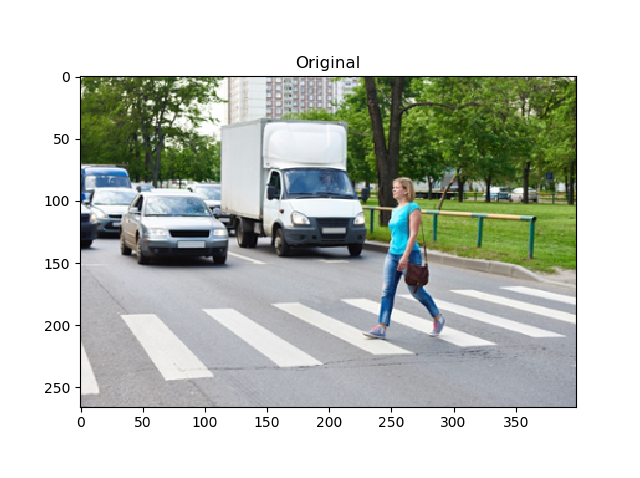
\includegraphics[width=80mm]{imagenes/prueba_1}}
	\subfigure{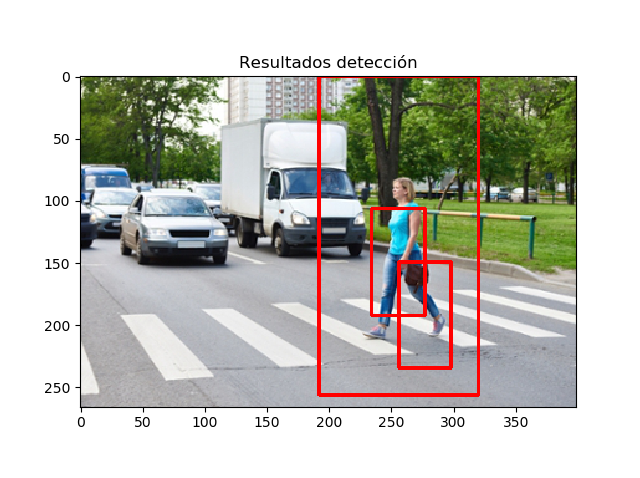
\includegraphics[width=80mm]{imagenes/resultado_1}}
	\caption{Prueba detección de personas 1}
	\label{fig:resultados1}
\end{figure}

\newpage

\begin{figure}[H]
	\centering
	\subfigure{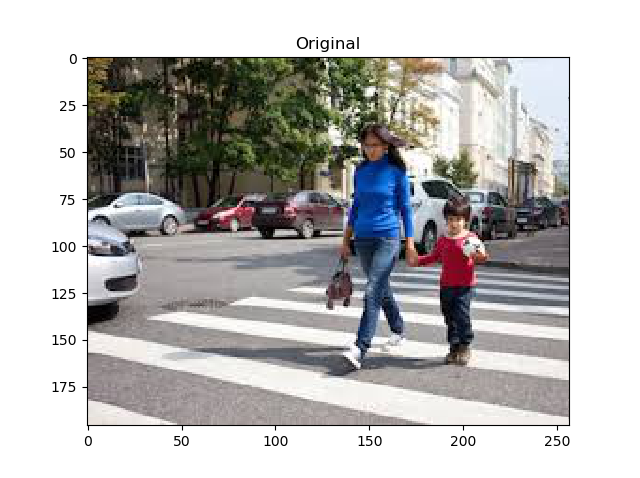
\includegraphics[width=80mm]{imagenes/prueba_2}}
	\subfigure{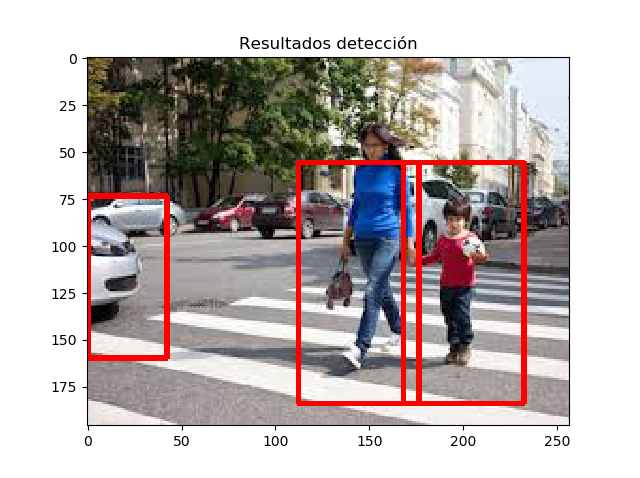
\includegraphics[width=80mm]{imagenes/resultado_2}}
	\caption{Prueba detección de personas 2}
	\label{fig:resultados2}
\end{figure}

\newpage

\begin{figure}[H]
	\centering
	\subfigure{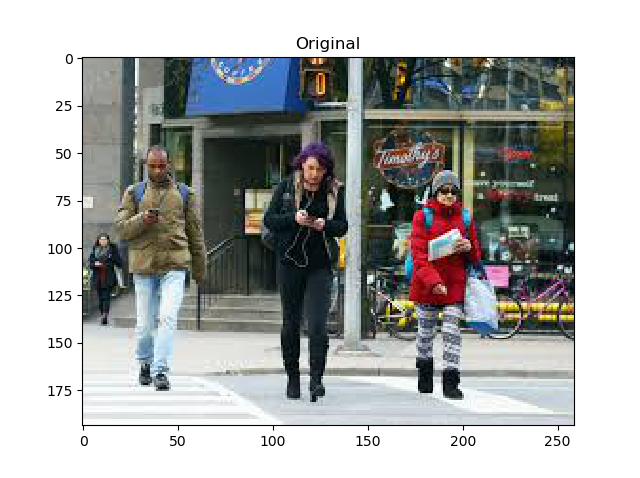
\includegraphics[width=80mm]{imagenes/prueba_3}}
	\subfigure{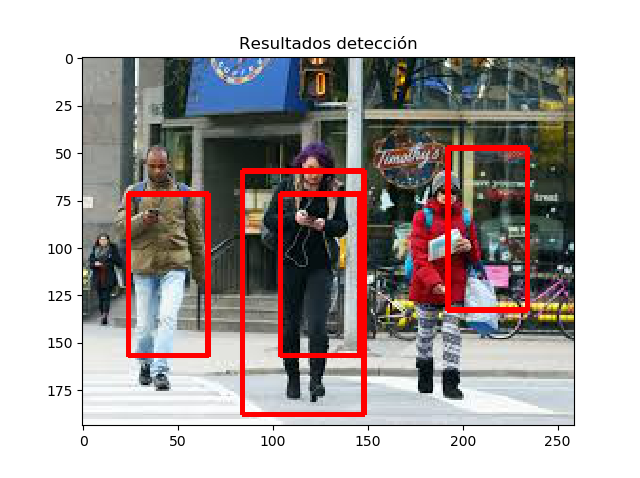
\includegraphics[width=80mm]{imagenes/resultado_3}}
	\caption{Prueba detección de personas 3}
	\label{fig:resultados3}
\end{figure}







\end{document}